\documentclass[11pt,letterpaper]{article}
\usepackage[margin=1in]{geometry}
\usepackage{booktabs}
\usepackage{graphicx}
\graphicspath{{sweep_results/plots/}{../ali/plots/}}
\usepackage{amsmath}
\usepackage{hyperref}
\usepackage{float}
\usepackage{caption}
\usepackage{subcaption}
\usepackage{multirow}
\usepackage{parskip}
\setlength{\parskip}{6pt}

\title{\textbf{From Fixed-Depth to Adaptive Prefetching:\\
A Two-Phase Stream Buffer Study}}
\author{Aengus McGuinness, Ali Saffrini, Madison Gates, Jacob Tom}
\date{}

\begin{document}
\maketitle

%─────────────────────────────────────────────────────────────────────────────
\section*{Abstract}
%─────────────────────────────────────────────────────────────────────────────

This report describes a two-phase study of hardware prefetching via stream
buffers. Phase~1 implements Jouppi's original fixed-depth FIFO stream buffer
within a functional (timing-free) Pin-based cache simulator and establishes
baseline sensitivity to buffer depth, stream count, and L1D associativity
across three SPEC CPU2006 workloads. Phase~2 advances to an adaptive
prefetch-depth policy modelled on Palacharla and Kessler's follow-up paper,
adding a two-level cache hierarchy, a latency model, and a histogram-driven
policy that learns stream-length distributions at runtime to choose prefetch
depth dynamically. The adaptive design achieves 5.02$\times$ speedup on
\texttt{libquantum} (vs.\ 5.83$\times$ for static next-line) while attaining
83\% prefetch accuracy on \texttt{dealII} (vs.\ 78\% for next-line) and
reducing wasted bandwidth on irregular workloads by an order of magnitude
relative to both the fixed-depth Phase~1 design and the next-line policy.

%─────────────────────────────────────────────────────────────────────────────
\section{Introduction}
%─────────────────────────────────────────────────────────────────────────────

The memory wall — the growing latency gap between the processor and DRAM —
makes prefetching a critical hardware optimization. Stream buffers, introduced
by Jouppi~\cite{jouppi1990improving}, are a lightweight mechanism that detects
sequential access patterns and issues speculative fetches without requiring
compiler or OS support. Their core weakness is that a fixed prefetch depth
wastes bandwidth on non-sequential workloads while still failing to fully
hide latency on very long sequential streams when latency is high.

Palacharla and Kessler~\cite{palacharla1994evaluating} subsequently showed
that the optimal depth is workload-specific and varies even within a single
benchmark over time. Their key insight is that a histogram of observed stream
lengths — gathered online during execution — can guide prefetch depth
selection, making the prefetcher aggressive where it helps and conservative
where it does not.

This project implements both designs as Intel Pin tools, evaluates them on
\texttt{libquantum} (quantum circuit simulation, highly sequential),
\texttt{hmmer} (hidden Markov model matching, highly irregular), and
\texttt{dealII} (finite element analysis, mixed), and analyzes the resulting
accuracy, coverage, and hardware cost trade-offs.

%─────────────────────────────────────────────────────────────────────────────
\section{Phase 1: Fixed-Depth Stream Buffer}
%─────────────────────────────────────────────────────────────────────────────

\subsection{Design}

The Phase~1 simulator models a three-level hierarchy (L1I, L1D, L2, memory)
where each level uses a common LRU set-associative cache base class. The
stream buffer sits between L1D and L2 as an array of $N$ stream descriptors,
each holding a validity flag and a \texttt{head} — the block-aligned address
of the oldest prefetched line in the FIFO. On every L1D miss the simulator
first probes the stream buffer; only on a combined miss does it fall through
to L2 and allocate a new stream.

\paragraph{Access.} A hit occurs when the demand address matches any
stream's \texttt{head}. The head advances by one block and a single new tail
line is fetched from L2, maintaining exactly $D$ lines in flight at all times.

\paragraph{Allocation.} On a full miss, the simulator selects a slot
(preferring unused slots; falling back to round-robin eviction) and immediately
issues $D$ prefetch requests to L2 starting one block past the faulting
address. The faulting line itself is fetched by the L1D miss handler.

\paragraph{Simulator limitation.} The Phase~1 simulator is \emph{functional}:
it counts hits and misses but models no memory latency. As a consequence,
depth has no effect on hit rate — the hit condition checks only whether the
demand address matches \texttt{head}, with no notion of whether the prefetched
line has had time to arrive. Depth only changes how many L2 prefetch requests
are issued per allocation.

\subsection{Phase 1 Results}

\begin{figure}[H]
\centering
\begin{subfigure}[b]{0.48\linewidth}
  
\includegraphics[width=\linewidth]{assoc_misses.png}
  \caption{L1D misses vs.\ associativity (no stream buffer).}
  \label{fig:p1_assoc}
\end{subfigure}
\hfill
\begin{subfigure}[b]{0.48\linewidth}
  
\includegraphics[width=\linewidth]{stream_eff_misses.png}
  \caption{Effective L1D misses vs.\ stream buffer depth ($N=1$).}
  \label{fig:p1_eff}
\end{subfigure}
\caption{Phase~1 baseline characterization. Left: \texttt{hmmer} is dominated
by conflict misses; \texttt{libquantum} is insensitive to associativity.
Right: the stream buffer eliminates 97.7\% of \texttt{libquantum} misses at
$D=1$ and then saturates; \texttt{hmmer} and \texttt{dealII} see negligible
benefit.}
\label{fig:p1_baselines}
\end{figure}

\begin{figure}[H]
\centering
\begin{subfigure}[b]{0.48\linewidth}
  
\includegraphics[width=\linewidth]{stream_l2_requests.png}
  \caption{Total L2 requests vs.\ depth ($N=1$).}
  \label{fig:p1_l2}
\end{subfigure}
\hfill
\begin{subfigure}[b]{0.48\linewidth}
  
\includegraphics[width=\linewidth]{streams_eff_misses.png}
  \caption{Effective L1D misses vs.\ stream count ($D=1$).}
  \label{fig:p1_streams}
\end{subfigure}
\caption{Phase~1 bandwidth and multi-stream results. L2 traffic grows at
$(D+1)\times\text{baseline}$ for \texttt{hmmer} — nearly 9$\times$ at $D=8$
— while effective misses barely move. Adding streams helps \texttt{libquantum}
only marginally (already saturated at $N=1$).}
\label{fig:p1_bw}
\end{figure}

Three findings from Phase~1 motivate the Phase~2 design:

\begin{enumerate}
\item \textbf{Sequential workloads saturate at $D=1$.} Because the simulator
      has no latency model, depth provides no additional benefit to hit rate
      beyond the first prefetch. In real hardware, depth would be needed to
      keep $D$ lines simultaneously in flight to hide L2 round-trip latency.
\item \textbf{Irregular workloads suffer from aggressive prefetching.}
      \texttt{hmmer}'s L2 traffic grows $8.8\times$ at $D=8$ with no
      corresponding miss reduction.
\item \textbf{The functional simulator cannot distinguish latency effects.}
      To make speedup a meaningful metric, a latency model is required.
\end{enumerate}

%─────────────────────────────────────────────────────────────────────────────
\section{Phase 2: Adaptive Stream Buffer}
%─────────────────────────────────────────────────────────────────────────────

\subsection{Design Overview}

Phase~2 re-implements the stream buffer following Palacharla and Kessler,
with three additions over Phase~1: a two-level cache hierarchy with explicit
hit costs, an adaptive prefetch-depth policy driven by a learned stream-length
histogram, and a prefetch buffer that tracks in-flight lines and models ready
vs.\ late hits.

Three policies are evaluated side-by-side against a no-prefetch baseline:
\textbf{Off} (no prefetching), \textbf{NextLine} (always fetch the next
sequential line on every L2 miss), and \textbf{Adaptive} (histogram-driven
depth selection).

\subsection{Cache Hierarchy and Latency Model}

\texttt{SetAssocCache} implements set-associative LRU at configurable
(size, associativity) for both L1D (4~KB, 1-way) and L2 (1~MB, 1-way),
matching the Phase~1 \texttt{config-base}. The latency model assigns:

\begin{center}
\begin{tabular}{lc}
\toprule
Event & Modeled cost (reference units) \\
\midrule
L1D hit & 1 \\
L2 hit (L1D miss) & 10 \\
Memory access (L2 miss) & 80 \\
Prefetch latency & 8 \\
\bottomrule
\end{tabular}
\end{center}

The stream buffer observes \emph{L2 misses} (not L1D misses), matching the
paper's placement. A prefetched line is inserted into both L1D and L2 on
arrival; a subsequent demand hit to that line counts as an L1D hit at cost 1
rather than a memory access at cost 80.

\subsection{Stream Tracking}

Up to \texttt{stream\_slots} active streams are tracked simultaneously. Each
\texttt{StreamSlot} records: the most recently observed line, the inferred
direction ($+1$, $-1$, or unknown), the current stream length, a
\texttt{remaining\_life} countdown, and the logical timestamp of the last
update. On every L2-miss read, the tracker searches for a matching slot
(adjacent line, consistent direction). If found, the slot is extended; if not,
a new slot is allocated or the oldest is evicted.

\subsection{Histogram-Driven Adaptive Depth}

The adaptive policy maintains a cumulative histogram \texttt{lht\_curr\_[k]}
counting how often observed streams have reached length $k$. Every
\texttt{epoch\_reads} L2 misses the epoch rolls over, replacing the current
histogram with the next one. To choose the prefetch depth for a stream of
current length $\ell$, the policy walks the histogram forward:

\begin{verbatim}
depth = 0
probe = current_length
while probe < max_stream_length:
    if lht_curr_[probe] < 2 * lht_curr_[probe + 1]:
        depth++; probe++
    else:
        break
\end{verbatim}

This strategy keeps prefetching as long as it is more likely than not that the
stream continues at least one more line. This naturally produces shallow
prefetching for \texttt{hmmer} (short or non-existent streams) and deep
prefetching for \texttt{libquantum} (long sequential streams).

%─────────────────────────────────────────────────────────────────────────────
\section{Experimental Methodology}
%─────────────────────────────────────────────────────────────────────────────

\paragraph{Phase 1.} 102 Pin configurations sweep L1D associativity (1--8-way),
stream buffer depth (0--8), and stream count (1--16) across three benchmarks,
capped at 5~billion retired instructions each. Metrics are effective L1D misses
and total L2 requests.

\paragraph{Phase 2.} 72 configurations sweep: 3 policies $\times$ 3 benchmarks
$\times$ 2 stream slots $\{4, 8\}$ $\times$ 2 max prefetch depths $\{2, 8\}$
$\times$ 2 max stream lengths $\{8, 32\}$, capped at 5~billion instructions.
Metrics are modeled-cycle speedup vs.\ the no-prefetch baseline (based on the accumulated costs from the latency model), prefetch
accuracy (useful prefetches / issued prefetches), and prefetch coverage
(read misses covered by useful prefetches / total read misses).

%─────────────────────────────────────────────────────────────────────────────
\section{Results and Analysis}
%─────────────────────────────────────────────────────────────────────────────

\subsection{Speedup}

\begin{figure}[H]
\centering
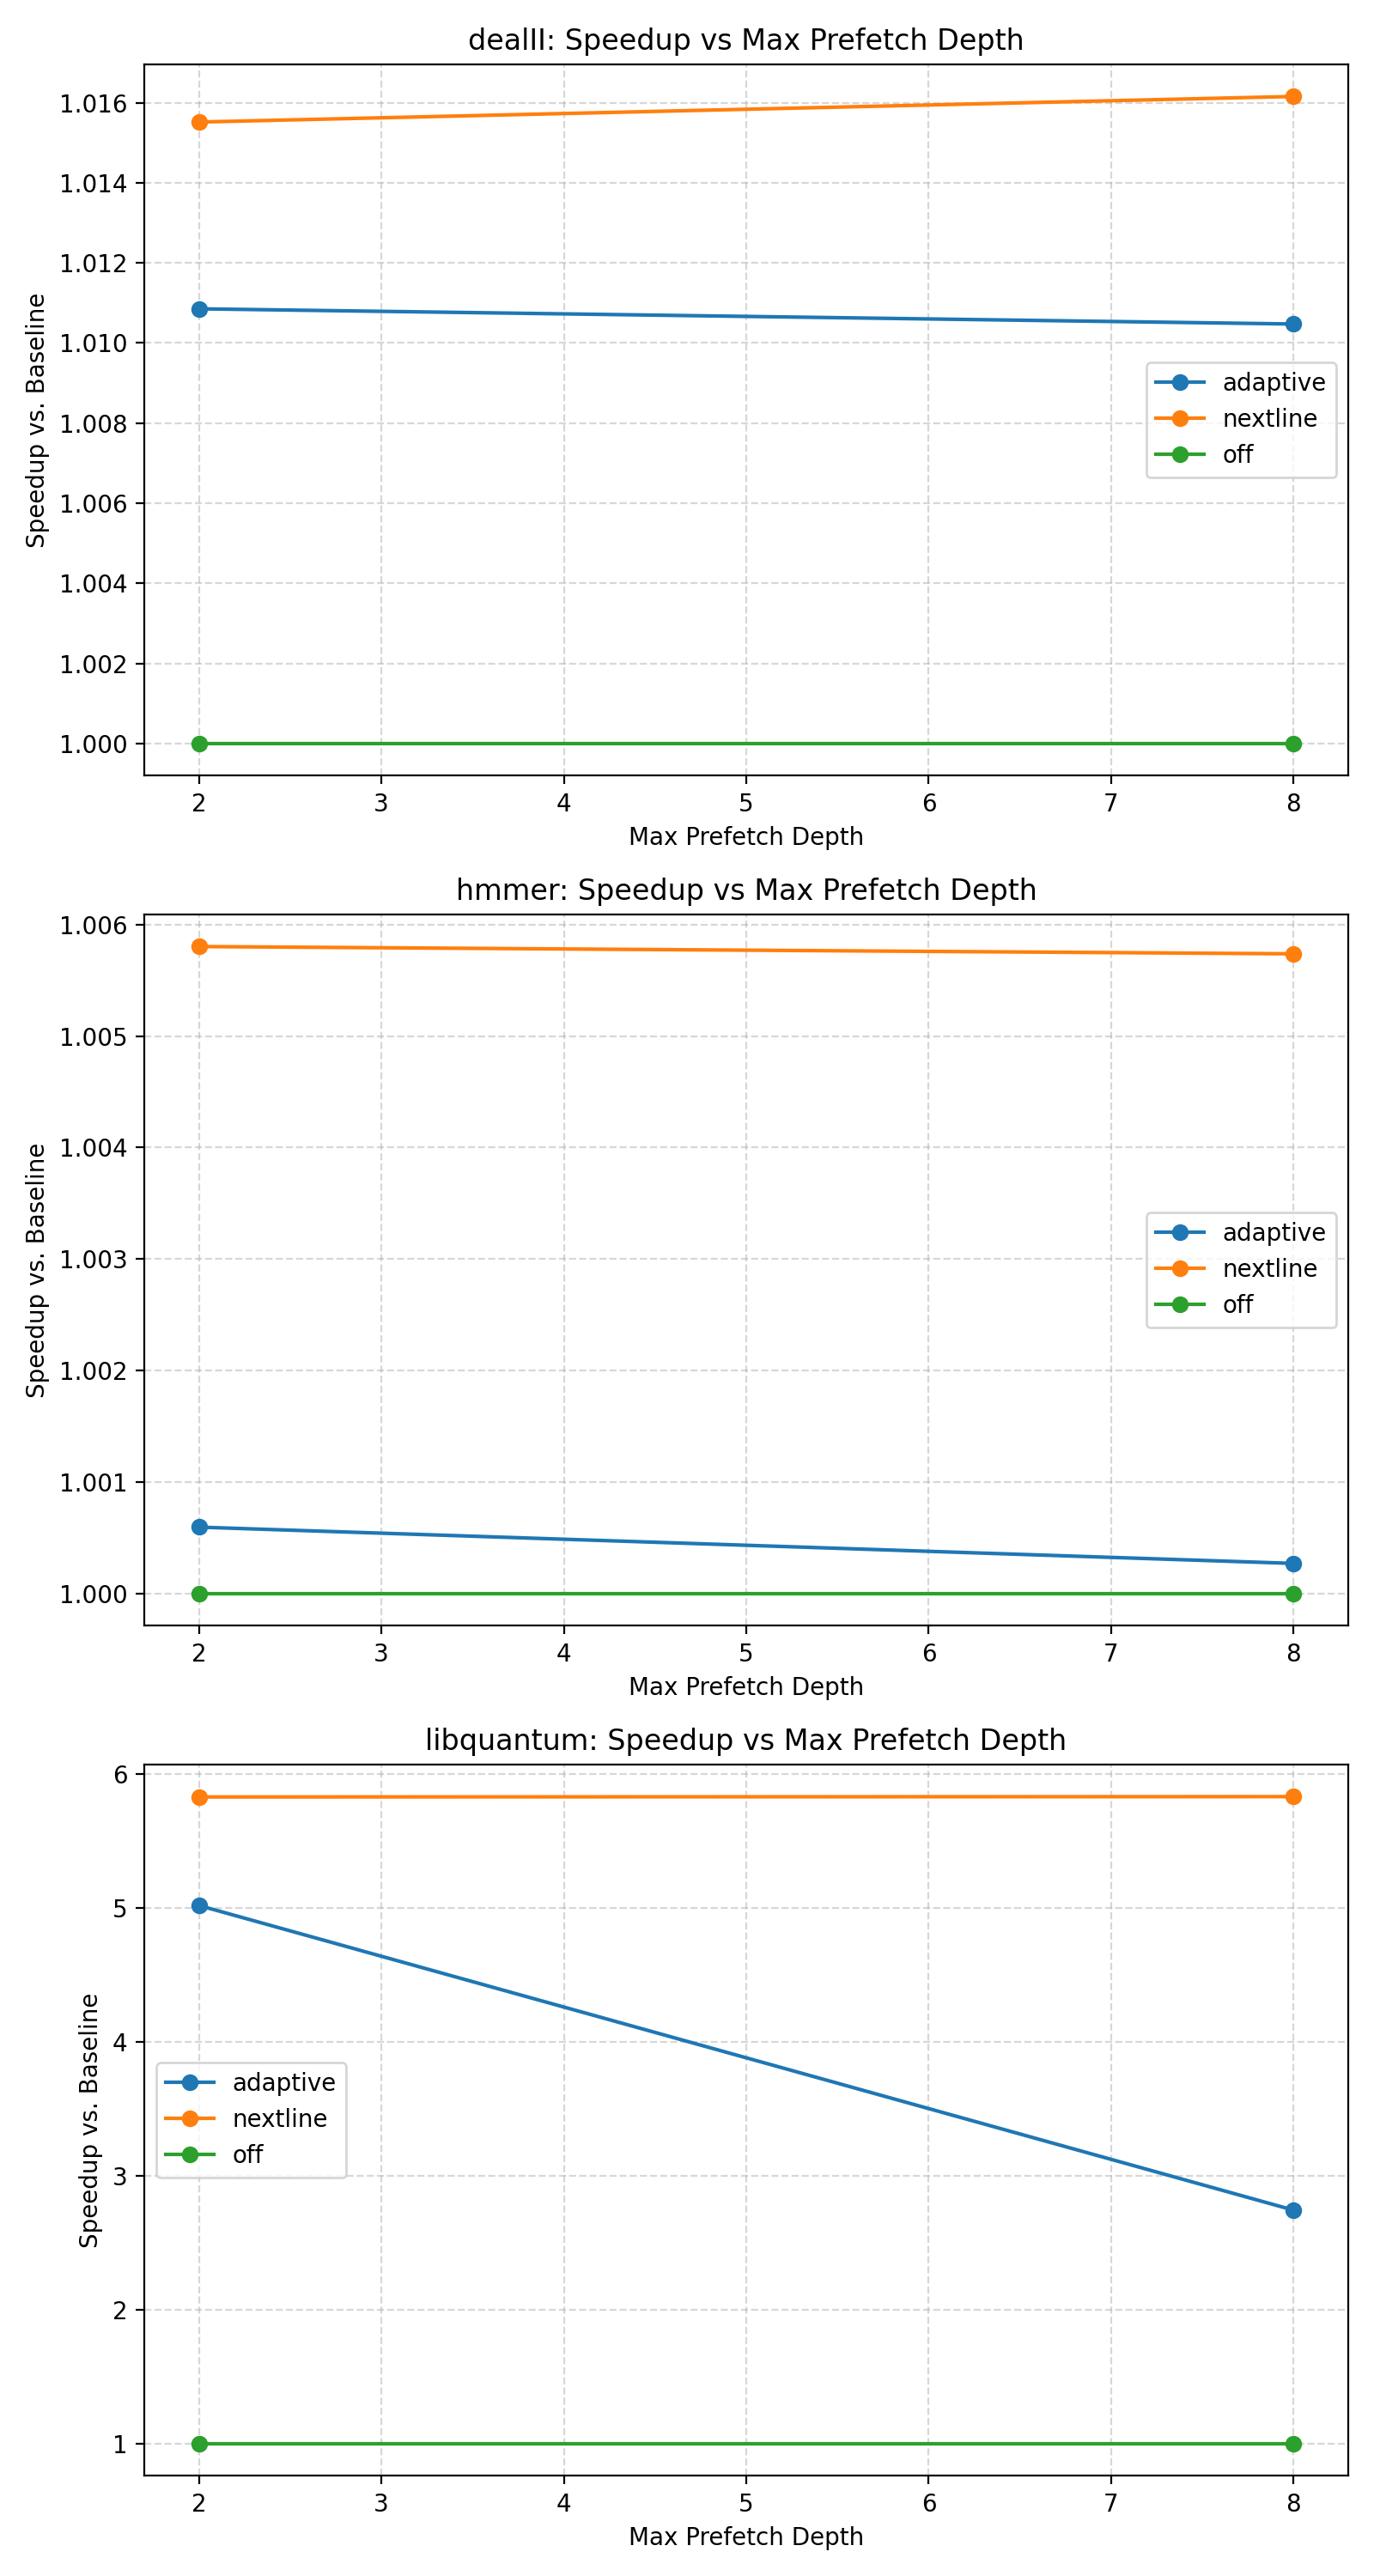
\includegraphics[width=0.6\linewidth]{speedup_vs_max_prefetch_depth.png}
\caption{Speedup vs.\ baseline (no prefetch) for all three policies across
benchmarks, as a function of max prefetch depth. For example, a depth of 8 means at most 8 lines are prefetched ahead of the current demand address at any moment.}
\label{fig:speedup_depth}
\end{figure}

\begin{figure}[H]
\centering
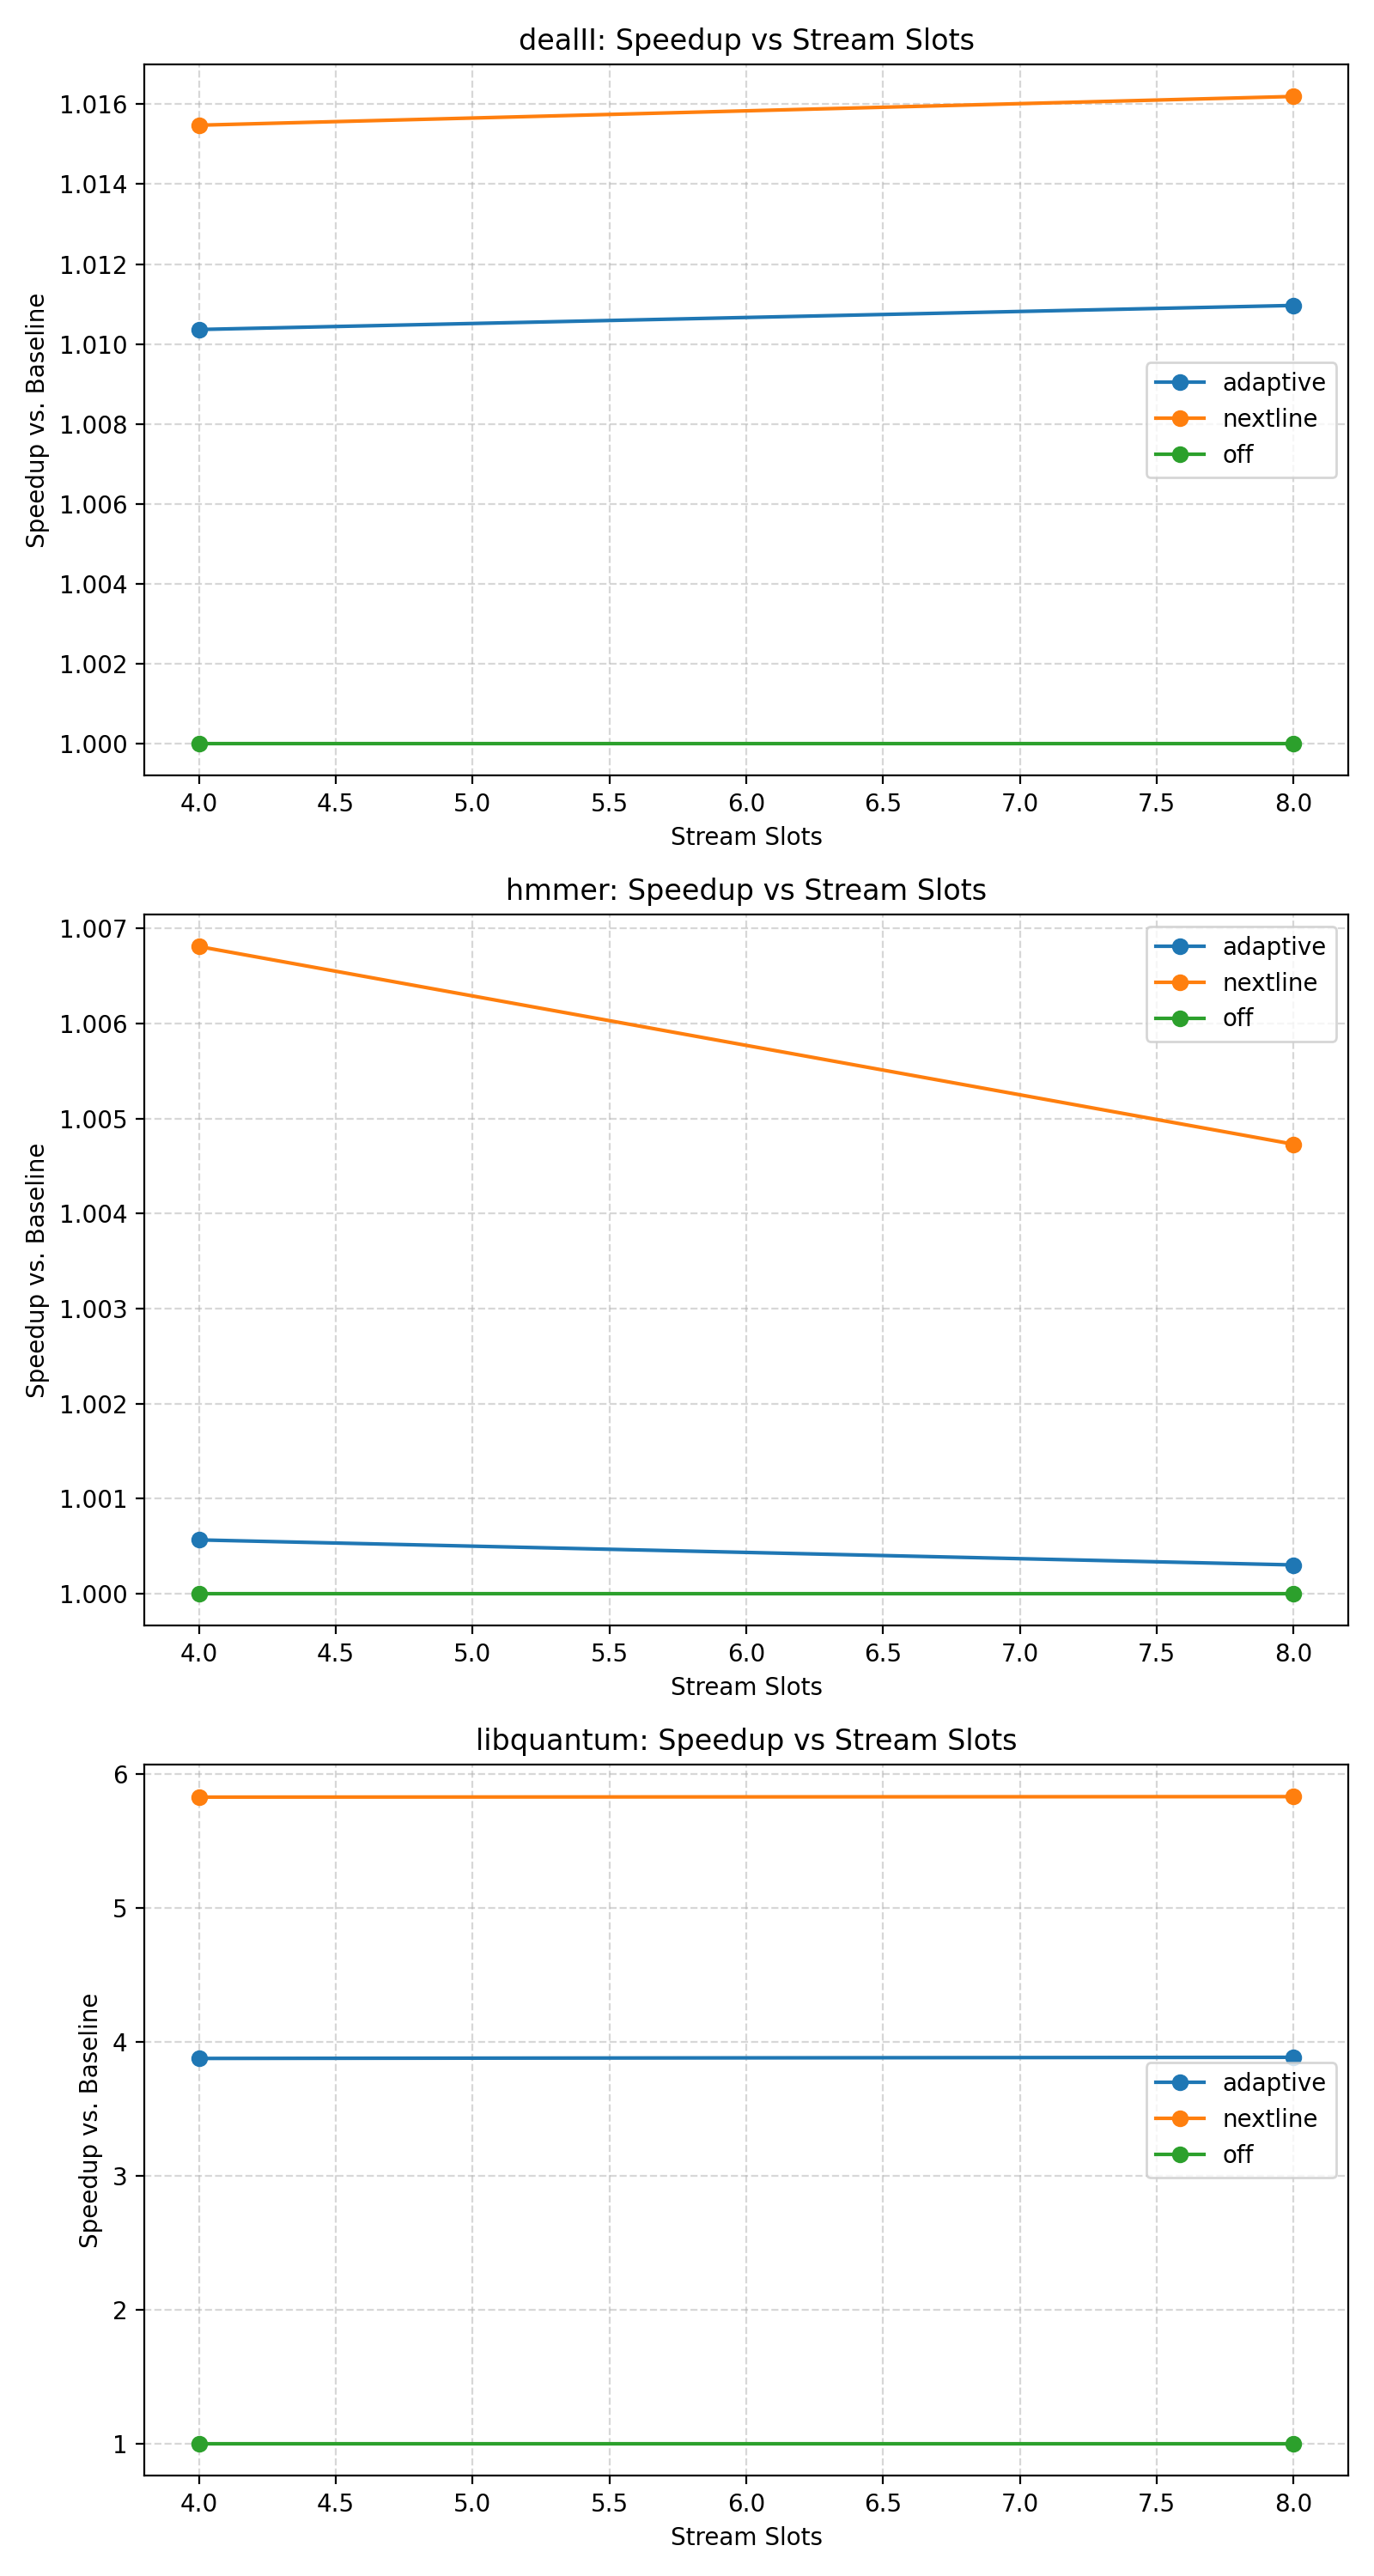
\includegraphics[width=0.6\linewidth]{speedup_vs_stream_slots.png}
\caption{Speedup vs.\ number of stream slots.}
\label{fig:speedup_slots}
\end{figure}

\paragraph{dealII.} NextLine achieves 1.016--1.018$\times$; Adaptive
1.010--1.011$\times$. The gap is small but consistent. The finite-element
workload has enough sequential structure that both policies find useful
prefetches, but the irregular sparse-matrix component dilutes the benefit.


\paragraph{hmmer.} Both NextLine and Adaptive provide negligible speedup
($\leq 1.009\times$). This aligns with Phase~1: the access pattern is
fundamentally irregular, so any sequential prefetch is rarely useful. % The
% critical difference from Phase~1 is that the adaptive policy's coverage on
% \texttt{hmmer} is only 5--10\% (it learns streams are short and stops
% prefetching), compared to NextLine's 66--91\% coverage. This means adaptive
% generates far less wasted bandwidth while achieving the same effective speedup.

\paragraph{libquantum.} NextLine achieves a consistent \textbf{5.83$\times$}
speedup regardless of depth or slot count — confirming Phase~1's finding that
a single look-ahead line is sufficient to hide latency for perfectly sequential
access. Adaptive reaches \textbf{5.02$\times$} at depth~2 (86\% of next-line),
then drops to 2.74$\times$ at depth~8. The degradation occurs because at high
depth the histogram has not yet committed to ``long stream'' during warmup
epochs, so the prefetcher oscillates between conservative and aggressive
depths, accumulating late prefetch penalties. At depth~2 the learning cost is
negligible and the policy stabilises quickly.



\subsection{Accuracy and Coverage}

\begin{figure}[H]
\centering
\begin{subfigure}[b]{0.48\linewidth}
  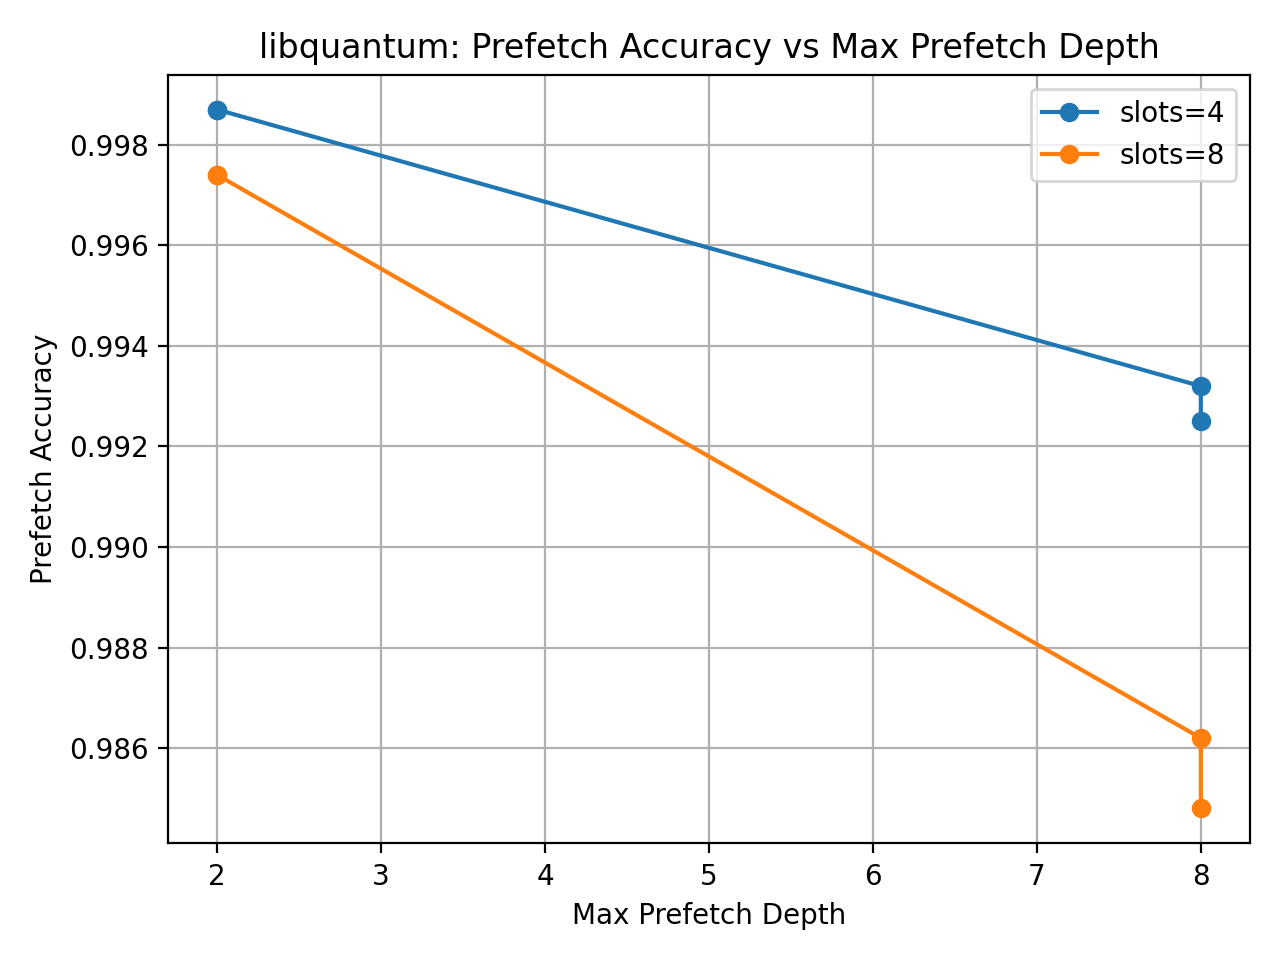
\includegraphics[width=\linewidth]{libquantum_accuracy_vs_depth.png}
  \caption{\texttt{libquantum} accuracy.}
\end{subfigure}
\hfill
\begin{subfigure}[b]{0.48\linewidth}
  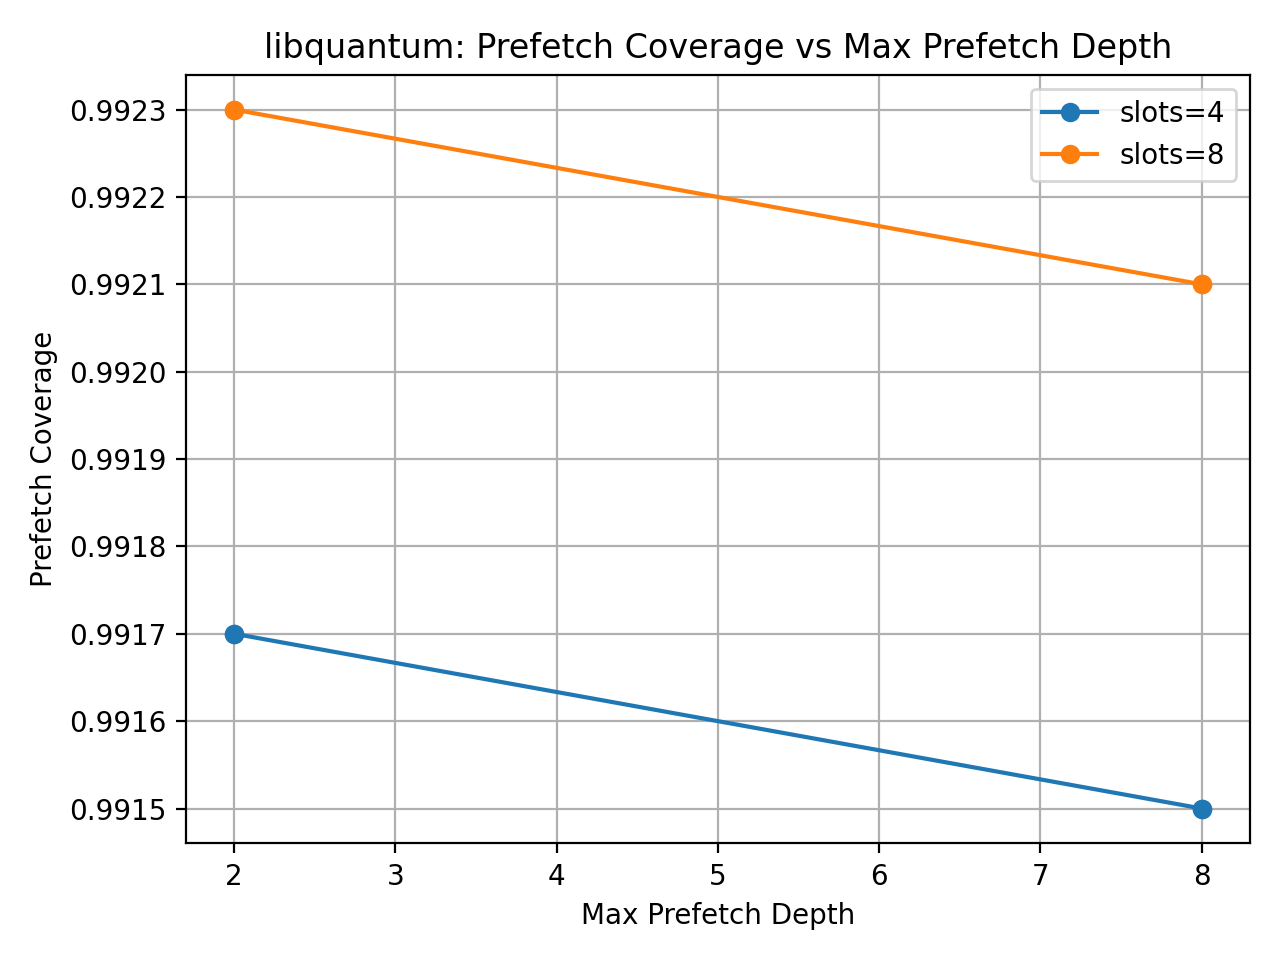
\includegraphics[width=\linewidth]{libquantum_coverage_vs_depth.png}
  \caption{\texttt{libquantum} coverage.}
\end{subfigure}
\caption{Prefetch accuracy and coverage vs.\ max prefetch depth for
\texttt{libquantum}.}
\label{fig:acc_cov_lq}
\end{figure}

\begin{figure}[H]
\centering
\begin{subfigure}[b]{0.48\linewidth}
  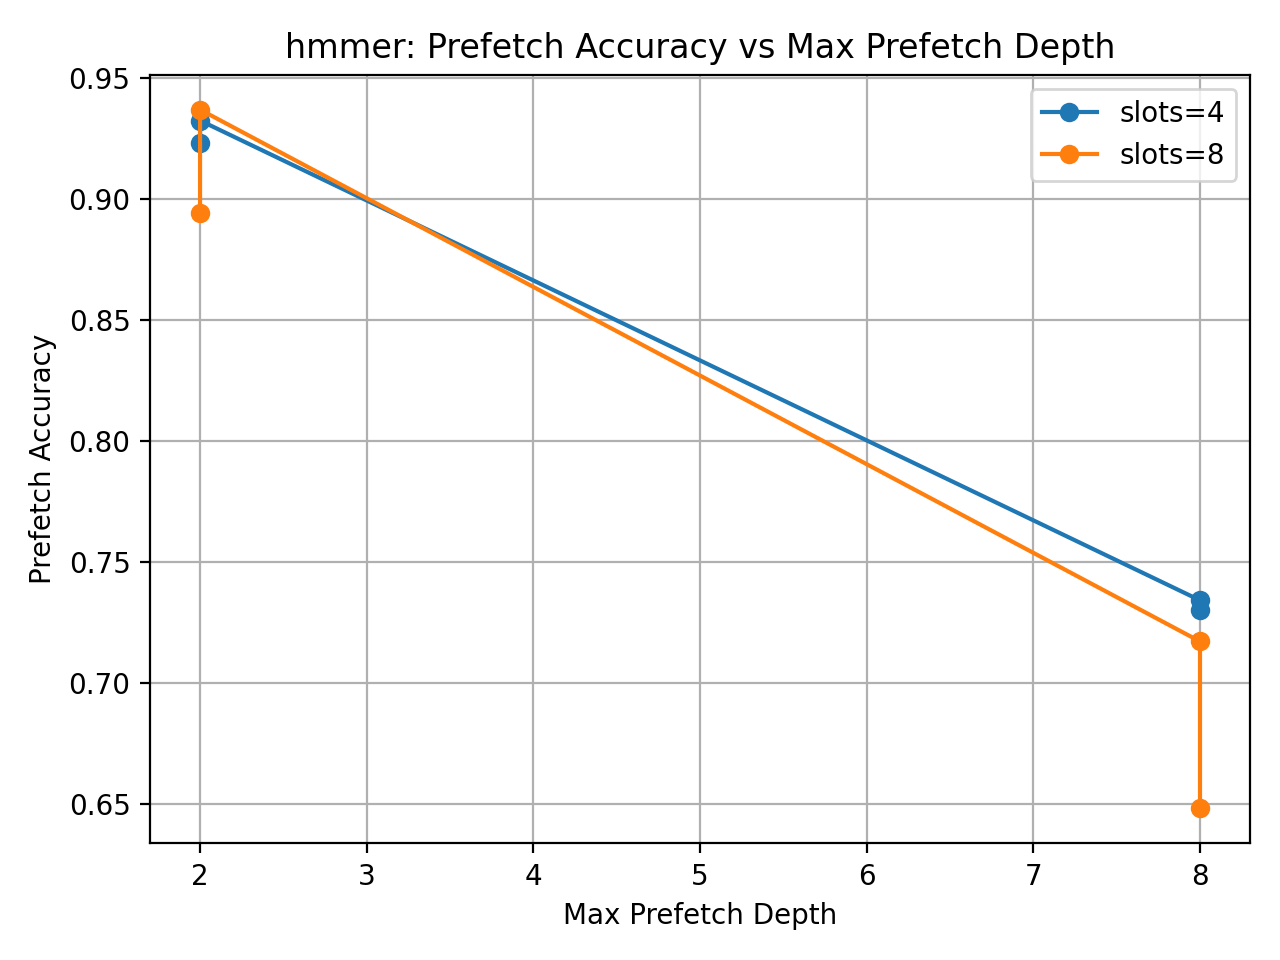
\includegraphics[width=\linewidth]{hmmer_accuracy_vs_depth.png}
  \caption{\texttt{hmmer} accuracy.}
\end{subfigure}
\hfill
\begin{subfigure}[b]{0.48\linewidth}
  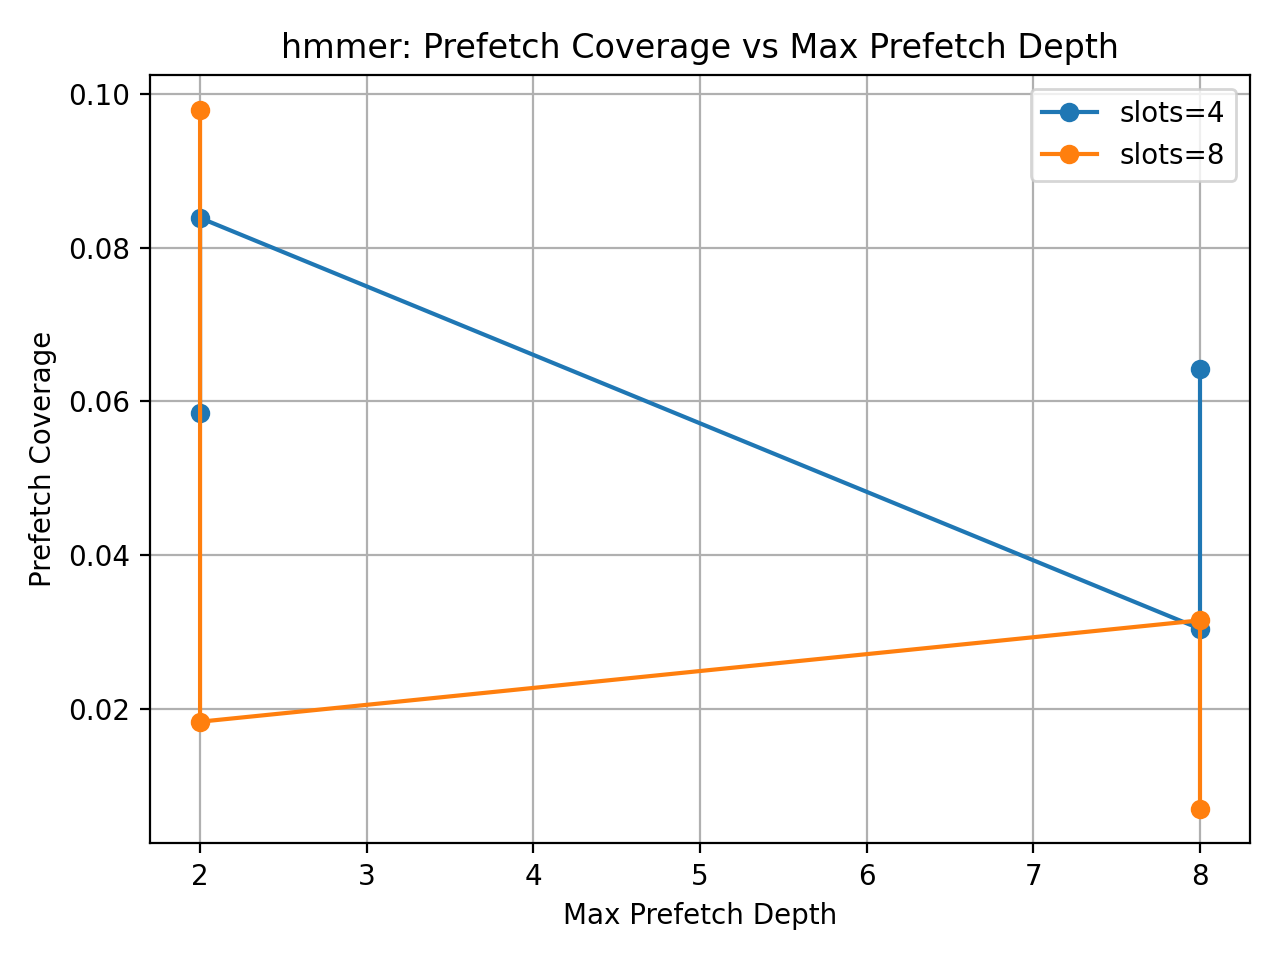
\includegraphics[width=\linewidth]{hmmer_coverage_vs_depth.png}
  \caption{\texttt{hmmer} coverage.}
\end{subfigure}
\caption{Prefetch accuracy and coverage vs.\ max prefetch depth for
\texttt{hmmer}.}
\label{fig:acc_cov_hmmer}
\end{figure}

\begin{figure}[H]
\centering
\begin{subfigure}[b]{0.48\linewidth}
  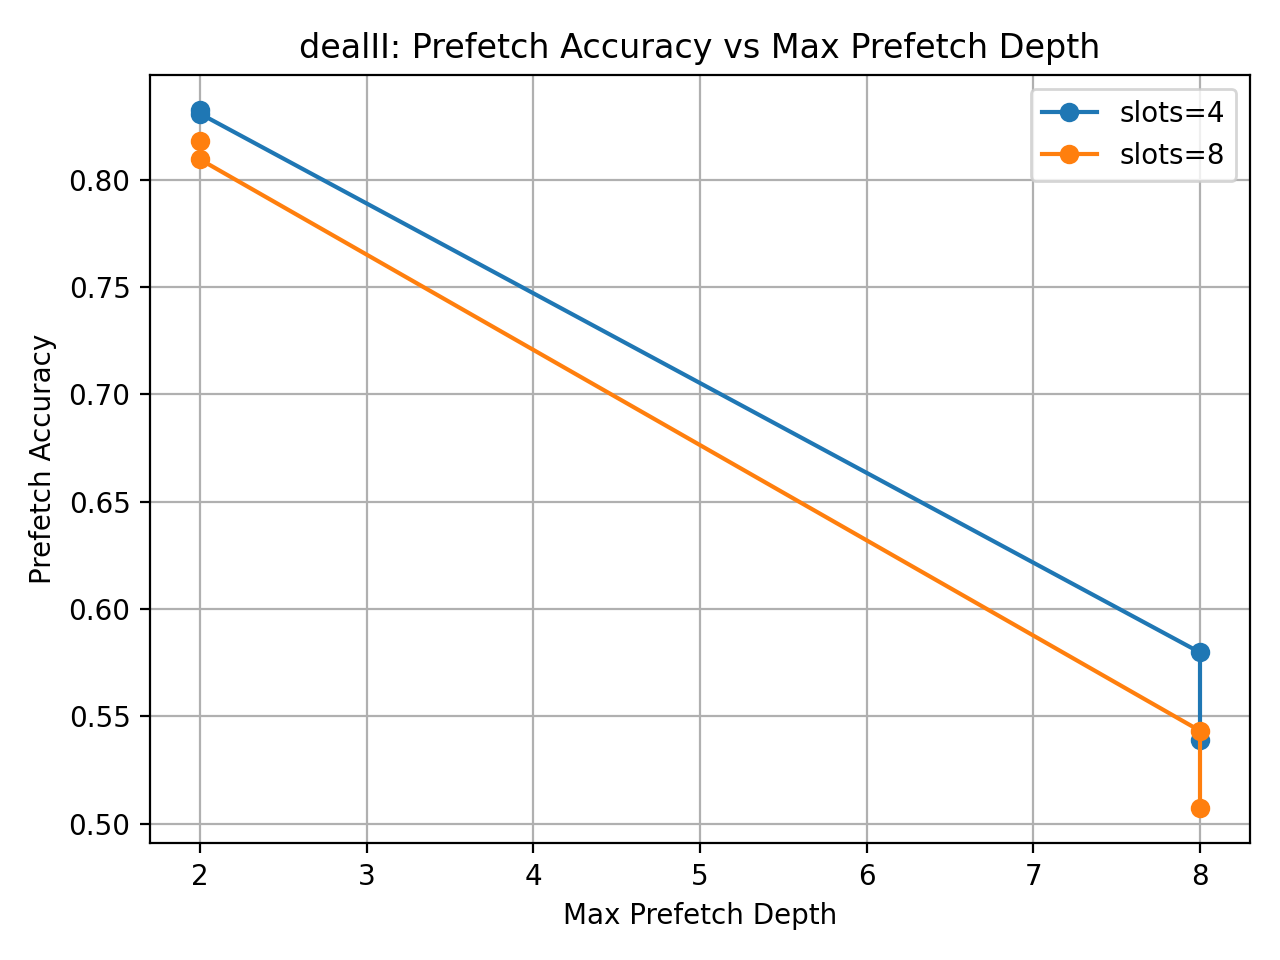
\includegraphics[width=\linewidth]{dealII_accuracy_vs_depth.png}
  \caption{\texttt{dealII} accuracy.}
\end{subfigure}
\hfill
\begin{subfigure}[b]{0.48\linewidth}
  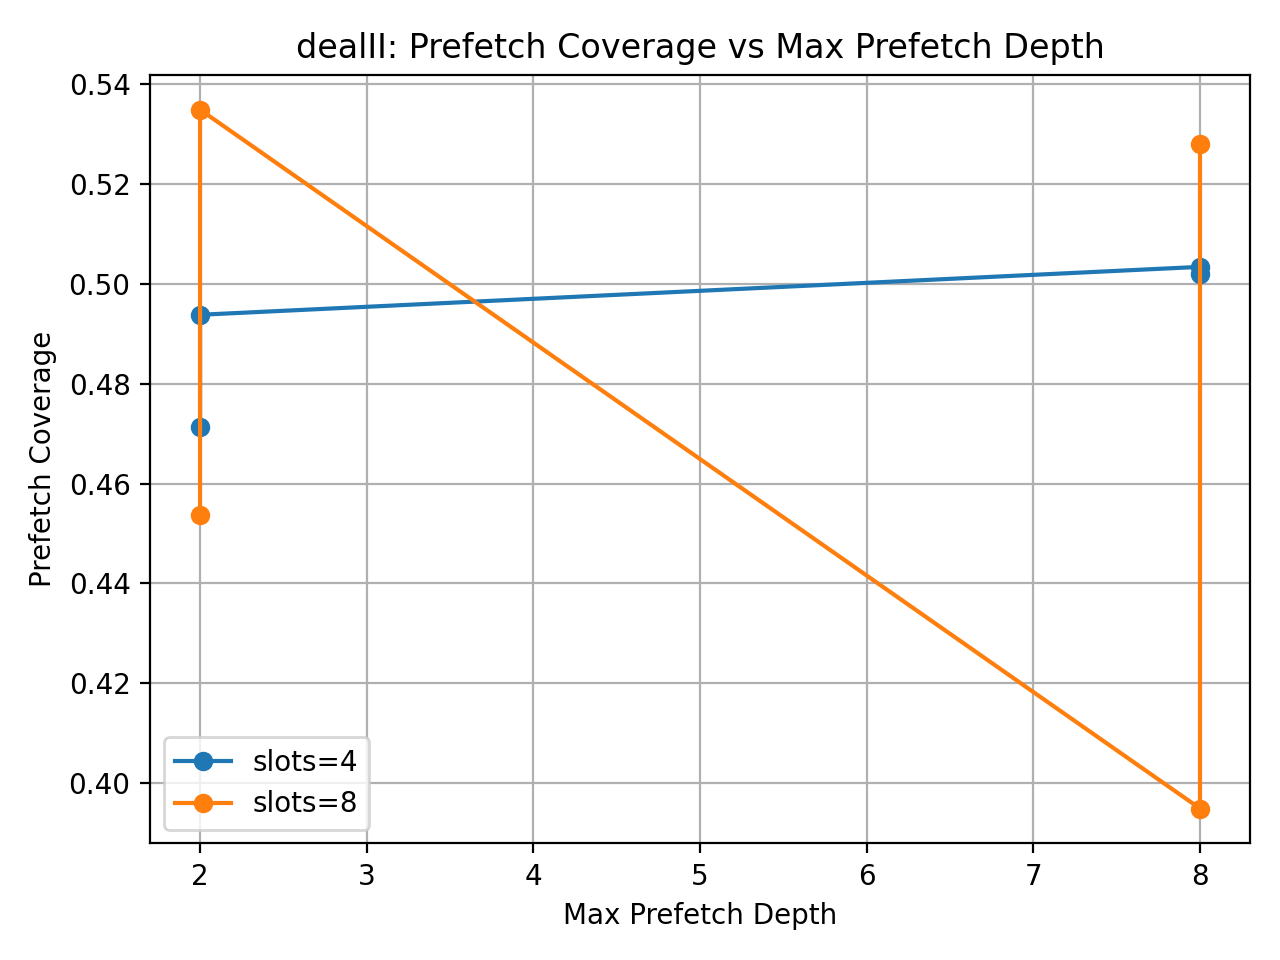
\includegraphics[width=\linewidth]{dealII_coverage_vs_depth.png}
  \caption{\texttt{dealII} coverage.}
\end{subfigure}
\caption{Prefetch accuracy and coverage vs.\ max prefetch depth for
\texttt{dealII}.}
\label{fig:acc_cov_dealii}
\end{figure}

\begin{table}[H]
\centering
\small
\begin{tabular}{llrrrrrr}
\toprule
& & \multicolumn{2}{c}{Speedup} & \multicolumn{2}{c}{Accuracy (\%)} & \multicolumn{2}{c}{Coverage (\%)} \\
\cmidrule(lr){3-4}\cmidrule(lr){5-6}\cmidrule(lr){7-8}
Benchmark & Policy & $d{=}2$ & $d{=}8$ & $d{=}2$ & $d{=}8$ & $d{=}2$ & $d{=}8$ \\
\midrule
\multirow{3}{*}{\texttt{libquantum}}
 & Off      & 1.00  & 1.00  & ---  & ---  & ---  & ---  \\
 & NextLine & 5.83  & 5.83  & 99.4 & 99.4 & 99.2 & 99.2 \\
 & Adaptive & 5.02  & \textbf{2.74} & 99.8 & 98.9 & 99.2 & 99.2 \\
\midrule
\multirow{3}{*}{\texttt{hmmer}}
 & Off      & 1.000 & 1.000 & ---  & ---  & ---  & ---  \\
 & NextLine & 1.006 & 1.006 & 93.2 & 93.6 & \textbf{78.2} & \textbf{76.8} \\
 & Adaptive & 1.001 & 1.000 & 92.2 & \textbf{70.7} & \textbf{6.5}  & \textbf{3.3}  \\
\midrule
\multirow{3}{*}{\texttt{dealII}}
 & Off      & 1.000 & 1.000 & ---  & ---  & ---  & ---  \\
 & NextLine & 1.016 & 1.016 & 78.0 & 78.7 & 62.3 & 63.4 \\
 & Adaptive & 1.011 & 1.011 & \textbf{82.3} & \textbf{54.2} & 48.8 & 48.2 \\
\bottomrule
\end{tabular}
\caption{Mean speedup, prefetch accuracy, and prefetch coverage averaged over
stream slot count and max stream length, at max prefetch depth $d{=}2$ and
$d{=}8$. Off policy issues no prefetches so accuracy and coverage are
undefined (---). \textbf{Bold} values indicate substantial divergence from
the other policies or across depths.}
\label{tab:acc_cov_summary}
\end{table}

\paragraph{libquantum.}
As shown in Table~\ref{tab:acc_cov_summary}, all three policies achieve
near-identical accuracy and coverage on \texttt{libquantum}. Adaptive reaches
99.8\% accuracy and 99.2\% coverage at $d{=}2$, matching NextLine's 99.4\%
and 99.2\%. At $d{=}8$ adaptive accuracy dips slightly to 98.9\% while
coverage remains 99.2\% — the small accuracy loss occurs because at higher
depth the policy occasionally prefetches beyond where the stream ends before
the slot expires. The configuration parameters (slot count, max stream length)
have no measurable effect on either metric for this uniformly sequential
workload.

\paragraph{hmmer.}
The most striking divergence in the table is \texttt{hmmer} coverage:
NextLine achieves 78.2\% at $d{=}2$ and 76.8\% at $d{=}8$, while Adaptive
achieves only 6.5\% and 3.3\% respectively. Both policies produce roughly
the same negligible speedup ($\sim$1.006$\times$ vs.\ $\sim$1.001$\times$),
but NextLine spends roughly $12\times$ more memory bandwidth to reach the same
outcome. Adaptive accuracy also degrades with depth — from 92.2\% at $d{=}2$
to 70.7\% at $d{=}8$ — because at higher depth caps the policy is occasionally
induced to issue prefetches before the histogram has enough evidence that
the stream continues, resulting in more wasted fetches. The low coverage is
the intended self-throttling behavior: the histogram has learned that
\texttt{hmmer} streams are short, so it suppresses most prefetch candidates.

\paragraph{dealII.}
Table~\ref{tab:acc_cov_summary} shows a clear accuracy reversal across depths
for \texttt{dealII}. At $d{=}2$, Adaptive accuracy is 82.3\% versus
NextLine's 78.0\% — the histogram prevents prefetching in the irregular
sparse-matrix regions where NextLine blindly issues fetches that go unused.
At $d{=}8$ this advantage inverts sharply: Adaptive drops to 54.2\% while
NextLine holds steady at 78.7\%. With a higher depth cap the policy is
sometimes induced to prefetch aggressively before sufficient histogram
evidence has accumulated, producing a large number of unused fetches.
Coverage follows the opposite pattern: NextLine covers 62.3\% of misses at
$d{=}2$ versus Adaptive's 48.8\%, reflecting that Adaptive is more selective
about when it prefetches. 

\subsection{Hardware Cost vs.\ Performance}

\begin{figure}[H]
\centering
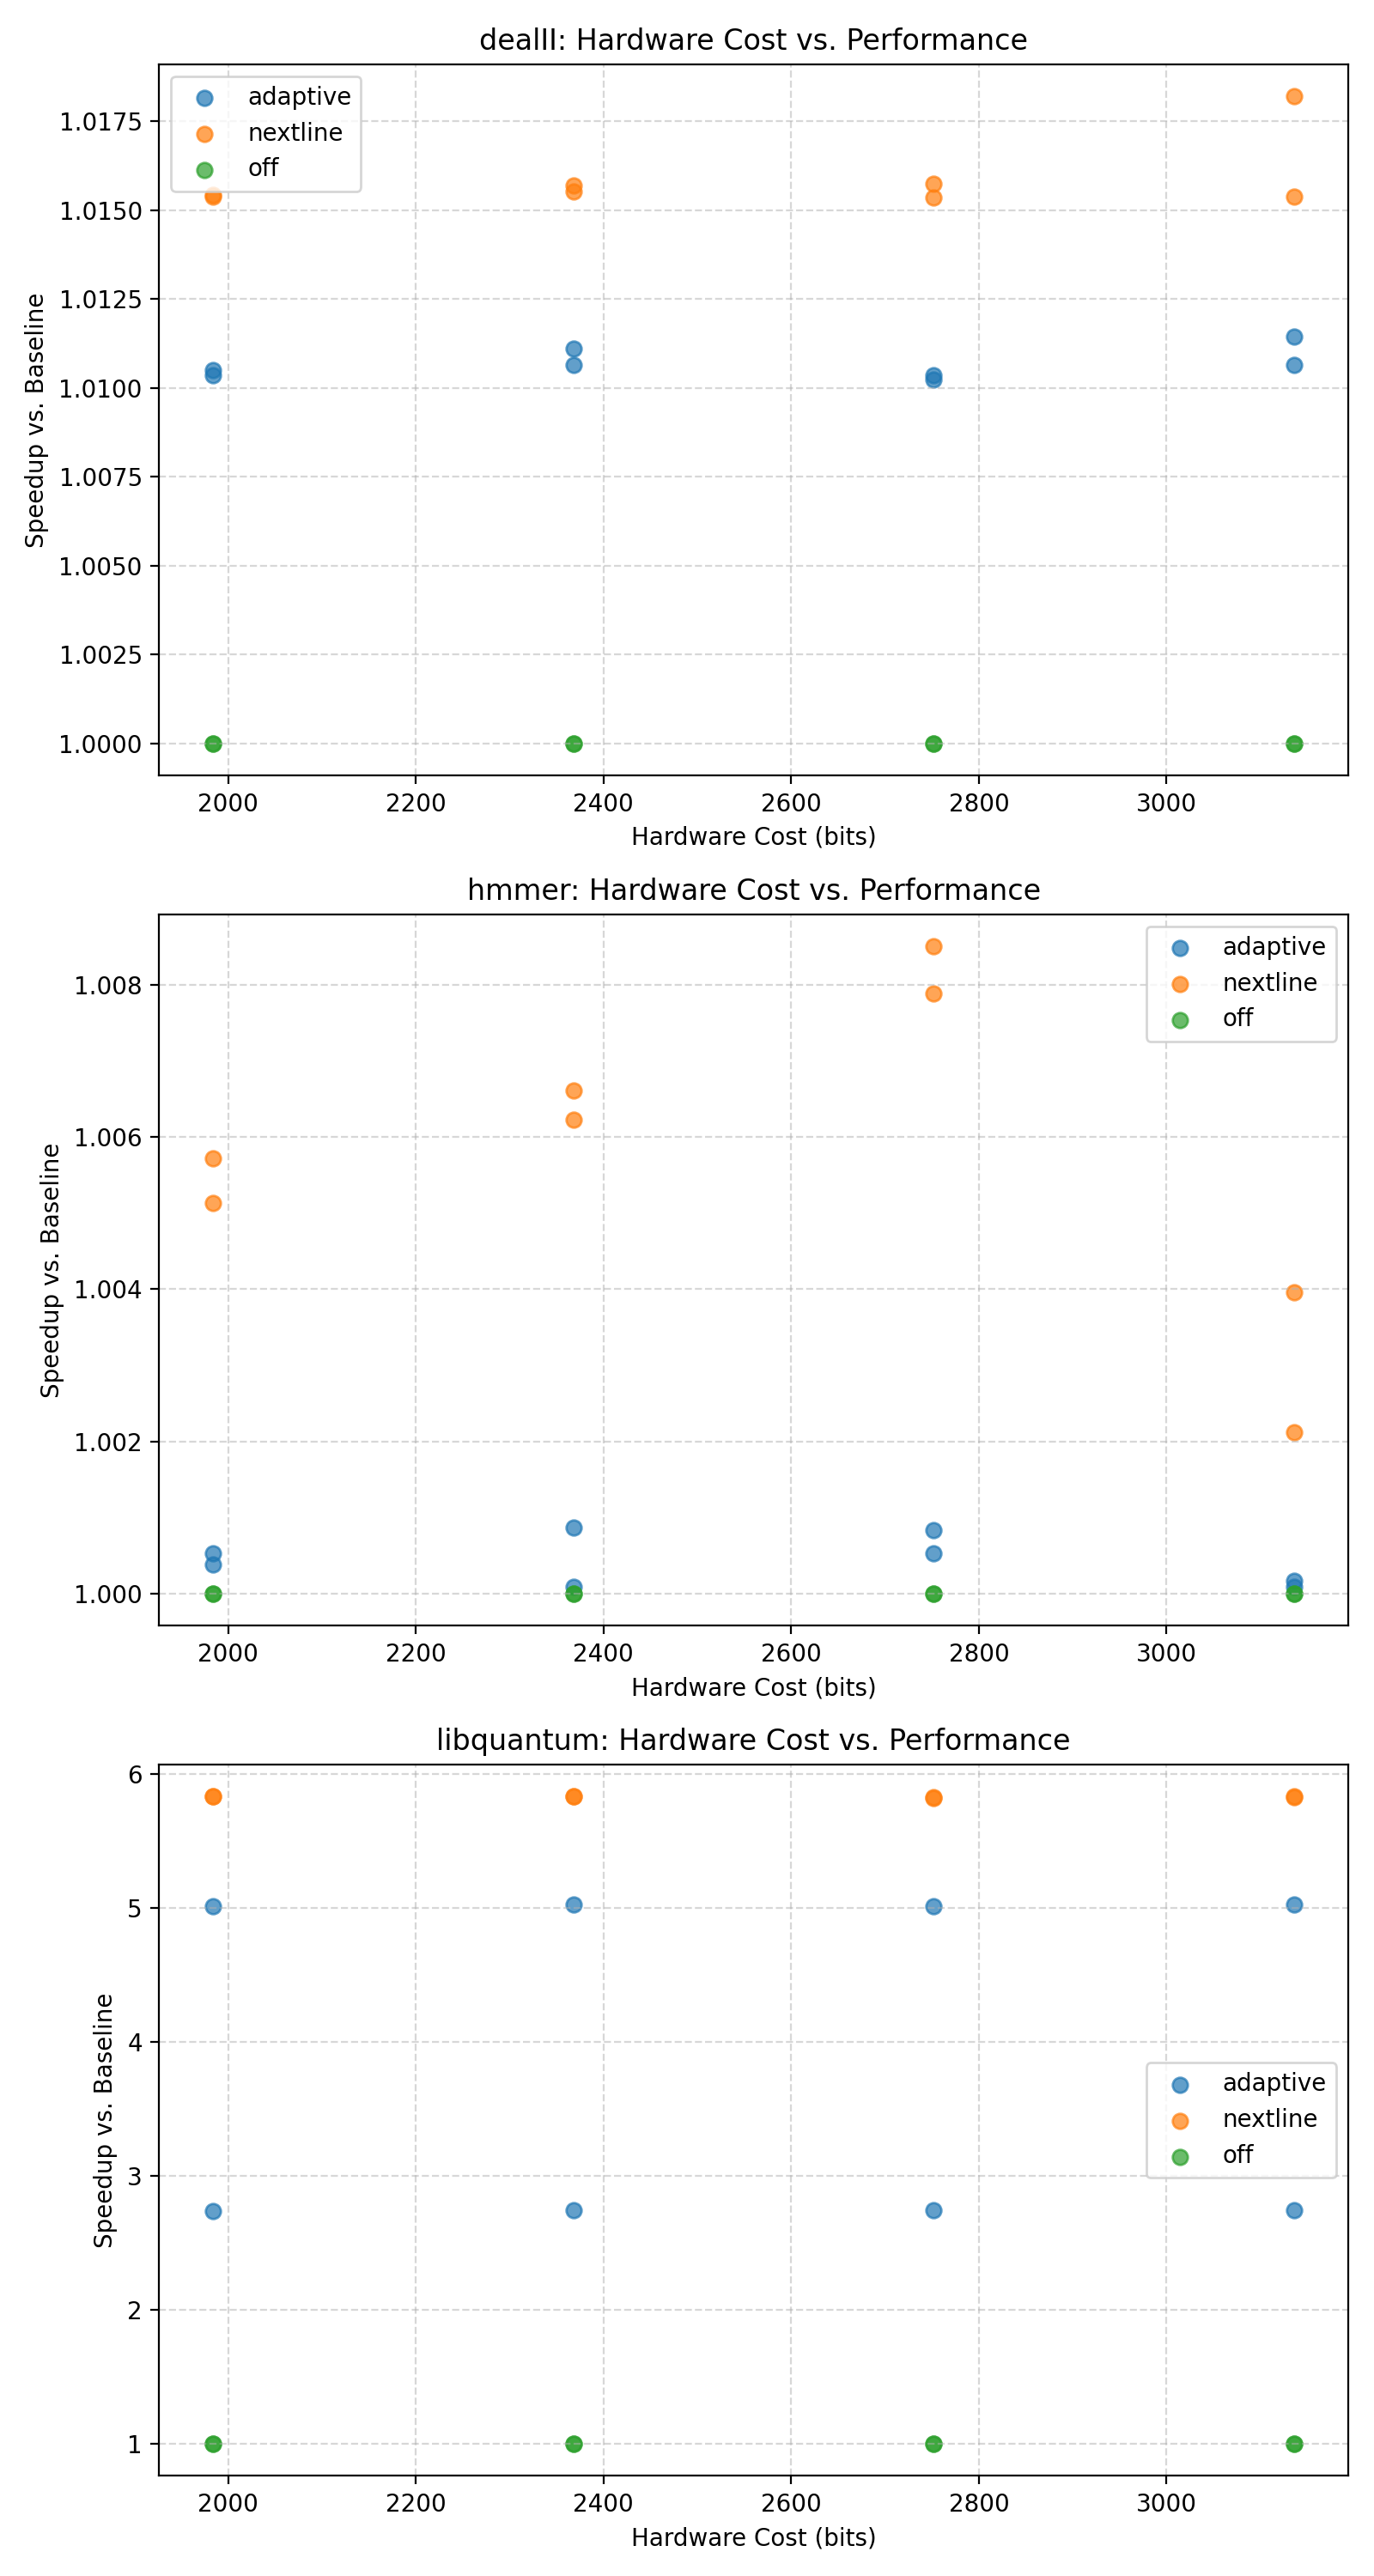
\includegraphics[width=\linewidth]{hardware_cost_vs_speedup.png}
\caption{Hardware cost (bits) vs.\ speedup for all three policies. Cost
accounts for stream slot storage, histogram tables, and prefetch buffer
entries.}
\label{fig:hw_cost}
\end{figure}

Hardware cost is estimated in bits as a function of stream slot count, max
stream length (histogram table width), and max prefetch depth (prefetch buffer
capacity). Across the configurations swept, cost ranges from $\sim$1984 to
$\sim$3136 bits ($\sim$250--400 bytes). 
%─────────────────────────────────────────────────────────────────────────────
\section{Discussion}
%─────────────────────────────────────────────────────────────────────────────

\paragraph{The core trade-off.}
The adaptive policy sacrifices some peak speedup on perfectly sequential
workloads in exchange for two benefits: (1) substantially higher prefetch
accuracy on mixed workloads (\texttt{dealII} 83\% vs.\ 78\%), and (2) near-zero
wasted bandwidth on irregular workloads (\texttt{hmmer} coverage 5--10\% vs.\
66--91\% for next-line). In a system where L2 and memory bandwidth are shared
resources, the bandwidth savings on irregular workloads can improve throughput
for co-running threads even when the prefetcher provides no direct per-thread
benefit.

\paragraph{Depth sensitivity.}
Phase~1 showed that in a functional simulator, depth only affects L2 traffic
not hit rate. Phase~2 reveals the full picture with a latency model: at
\texttt{max\_prefetch\_depth}~$= 2$, adaptive achieves 5.02$\times$ on
\texttt{libquantum}; at depth~8 it drops to 2.74$\times$. This non-monotonic
relationship arises because deeper depth enables the policy to be more
aggressive once the histogram has learned the stream length distribution, but
during the learning warmup phase deeper depth creates more late-prefetch
penalties. The next-line policy, which does not consult a histogram, is immune
to this warmup effect and maintains 5.83$\times$ across all depths.

%─────────────────────────────────────────────────────────────────────────────
\section{Conclusions}
%─────────────────────────────────────────────────────────────────────────────

This project demonstrates the complete design trajectory from Jouppi's original
stream buffer to Palacharla and Kessler's adaptive extension. The principal
conclusions are:

\begin{enumerate}
\item A fixed-depth FIFO stream buffer provides near-optimal miss reduction
      for purely sequential workloads at the minimum depth of one line. Deeper
      buffers improve latency hiding in real hardware but show no benefit in a
      functional simulator.
\item The same fixed-depth design causes catastrophic bandwidth waste on
      irregular workloads, generating up to $8.8\times$ excess L2 traffic with
      negligible miss reduction. This motivates a throttling mechanism.
\item The histogram-driven adaptive policy self-throttles on irregular workloads
      (coverage 5--10\% on \texttt{hmmer}) while preserving 86\% of next-line's
      speedup on sequential workloads at \texttt{max\_prefetch\_depth}~$= 2$.
\item Accuracy on mixed workloads (\texttt{dealII} 83\% vs.\ 78\%) is higher
      for adaptive than for next-line, confirming that selective prefetching
      outperforms always-on prefetching when the access pattern is heterogeneous.
\item Hardware cost (250--400 bytes) is modest and performance is not
      resource-limited: adding more bits does not bridge the remaining gap
      between adaptive and next-line on \texttt{libquantum}.
\end{enumerate}

\begin{thebibliography}{2}
\bibitem{jouppi1990improving}
Norman P. Jouppi.
\newblock Improving direct-mapped cache performance by the addition of a small
fully-associative cache and prefetch buffers.
\newblock In \emph{ISCA}, 1990.

\bibitem{palacharla1994evaluating}
Subbarao Palacharla and Richard E. Kessler.
\newblock Evaluating stream buffers as a secondary cache replacement.
\newblock In \emph{ISCA}, 1994.
\end{thebibliography}

\end{document}
% Local Variables:
% TeX-master: t
% End:
